\documentclass[tikz,border=10pt]{standalone}
\usepackage{tikz}
\usetikzlibrary{scopes}
\usepackage{verbatim}
\usetikzlibrary{calc,angles,patterns,quotes}
\usepackage{pgfplots}
\usepackage{pgf}
\pgfplotsset{compat=newest}
\pgfplotsset{plot coordinates/math parser=false}


\begin{document}

\def\iangle{35} % Angle of the inclined plane
\def\down{-90}
\def\arcr{0.5cm} % Radius of the arc used to indicate angles
\def\ang{30}
\def\rodlength{1}
\def\soundspeed{1}

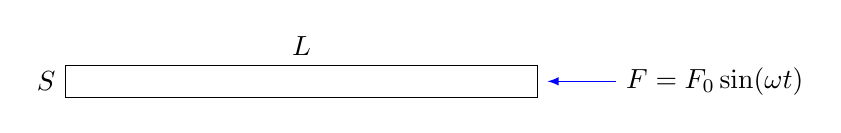
\begin{tikzpicture}[
    force/.style={>=latex,draw=blue,fill=blue},
    axis/.style={densely dashed,gray},
    M/.style={rectangle,draw,fill=lightgray,minimum size=0.5cm,thin},
    m/.style={rectangle,draw=black,fill=lightgray,minimum size=0.3cm,thin},
    plane/.style={draw=black,fill=blue!10},
    string/.style={draw=red, thick},
    pulley/.style={thick}
]


   
    % object and forces acting on it
    \draw (0cm, 0cm) rectangle ++(6cm, 0.4cm) -- ++(0, -0.2cm) node (right_edge){};
    \node[anchor=south] at (3cm, 0.4cm) {$L$};
    \node[anchor=east] at (0cm, 0.2cm) {$S$};

    \draw[force,>=latex,<-] (right_edge) -- ++(1, 0) node[right] {$F=F_0 \sin (\omega t)$};
   


\end{tikzpicture}
